This chapter describes and discusses the results of the running time measurements of the cluster and baseline implementations as described in \ref{chap:implementation}.
\section{ListNet}
Figure \ref{fig:listnet_train_time} and Figure \ref{fig:listnet_train_time_log} (which presents the same data with a logarithmic data size axis) show the processing times of a single training iteration using the ListNet implementation included in RankLib library and the cluster implementation described in chapter \ref{chap:implementation} with different numbers of data nodes. The horizontal positions of the measurements are identical between execution method, as they are determined by the collection of datasets used. As previously described in the methodology section, the LETOR 3.0, LETOR 4.0 and MSLR-WEB10/30K datasets are used, supplemented with generated datasets that are multiplications of MSLR-WEB30K. Table \ref{tbl:recap_datasets} describes the datasets used in the experiments.

\begin{table}[!h]
\centering
\begin{tabular}{p{3.4cm}p{3.4cm}r}\toprule
Dataset & Collection & Size \\
\midrule
MINI		& GENERATED		  & 143.38 KB\\
OHSUMED     & LETOR 3.0       &   4.55 MB\\
MQ2008      & LETOR 4.0       &   5.93 MB\\
MQ2007      & LETOR 4.0       &  25.52 MB\\
MSLR-WEB10K & MSLR-WEB10K     & 938.01 MB\\
MSLR-WEB30K & MSLR-WEB30K     &   2.62 GB\\
CUSTOM-2	& GENERATED		  &   5.25 GB\\
CUSTOM-5	& GENERATED		  &  13.12 GB\\
CUSTOM-10	& GENERATED		  &  26.24 GB\\
CUSTOM-20   & GENERATED       &  52.42 GB\\
CUSTOM-50	& GENERATED		  & 131.21 GB\\
CUSTOM-100	& GENERATED		  & 262.41 GB\\
\bottomrule
\end{tabular}
\caption{Description of datasets used for running time experiments}
\label{tbl:recap_datasets}
\end{table}

Figures \ref{fig:listnet_train_time} and \ref{fig:listnet_train_time_log} show that the single-machine RankLib implementation of ListNet is very fast compared to the Hadoop MapReduce cluster implementation of ListNet for datasets that fit in memory. As soon as the amount of data processed with RankLib ListNet approaches the physical memory limit of the machine used for the computation (16 GB for the machine used in our experiments), RankLib ListNet processing time start to increase very rapidly. This increase is likely to be a result of swapping data to and from virtual memory. The largest dataset processed with RankLib ListNet is CUSTOM-8, which is 20.99 GB in size and therewith larger than the 16 GB physical memory limit. Experiments with RankLib ListNet on CUSTOM-10 were attempted, but were stopped after not completing within 12 hours.\\

\begin{figure}[!h]
\centering
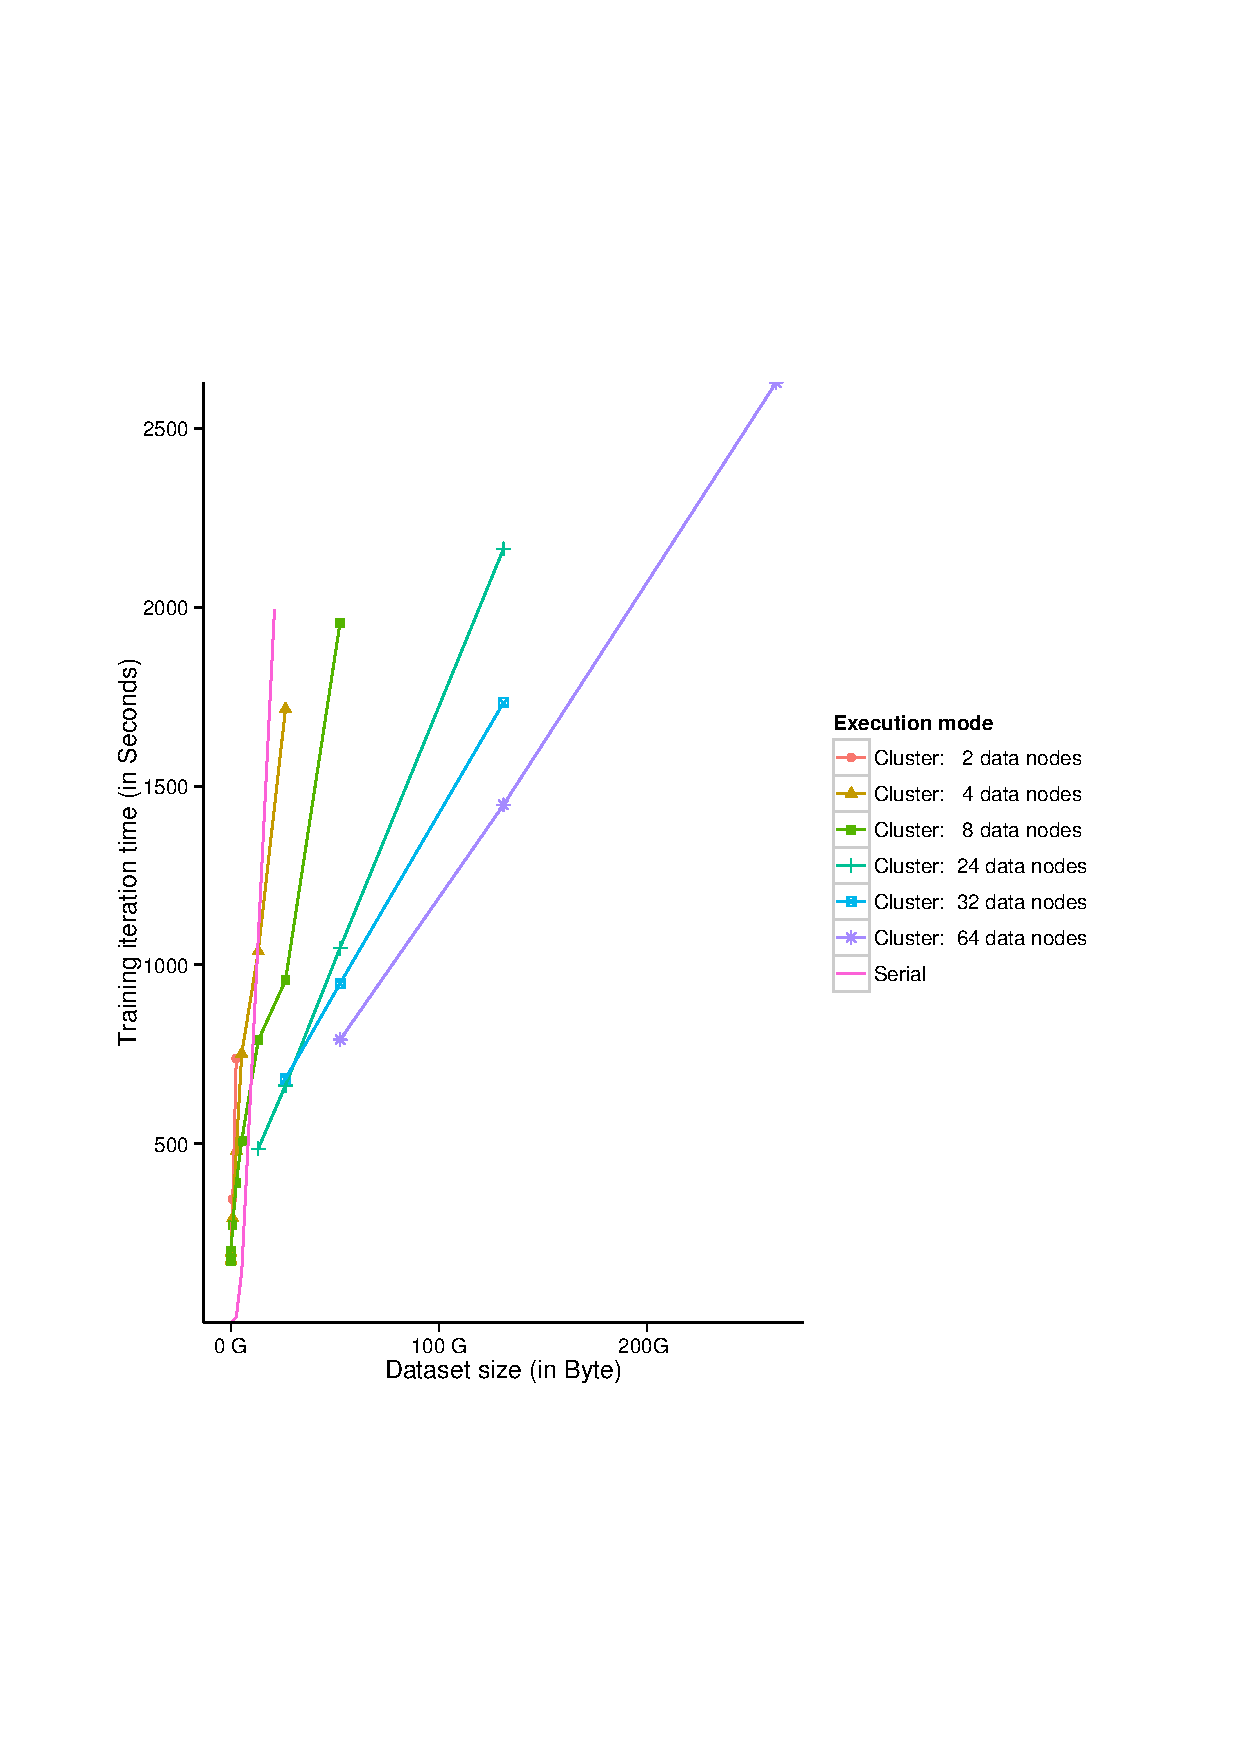
\includegraphics[trim=0cm 5cm 0cm 5cm, scale=0.8]{gfx/time_single.pdf}
\caption{Processing time of a single ListNet training iteration}
\label{fig:listnet_train_time}
\end{figure}

\begin{figure}[!h]
\centering
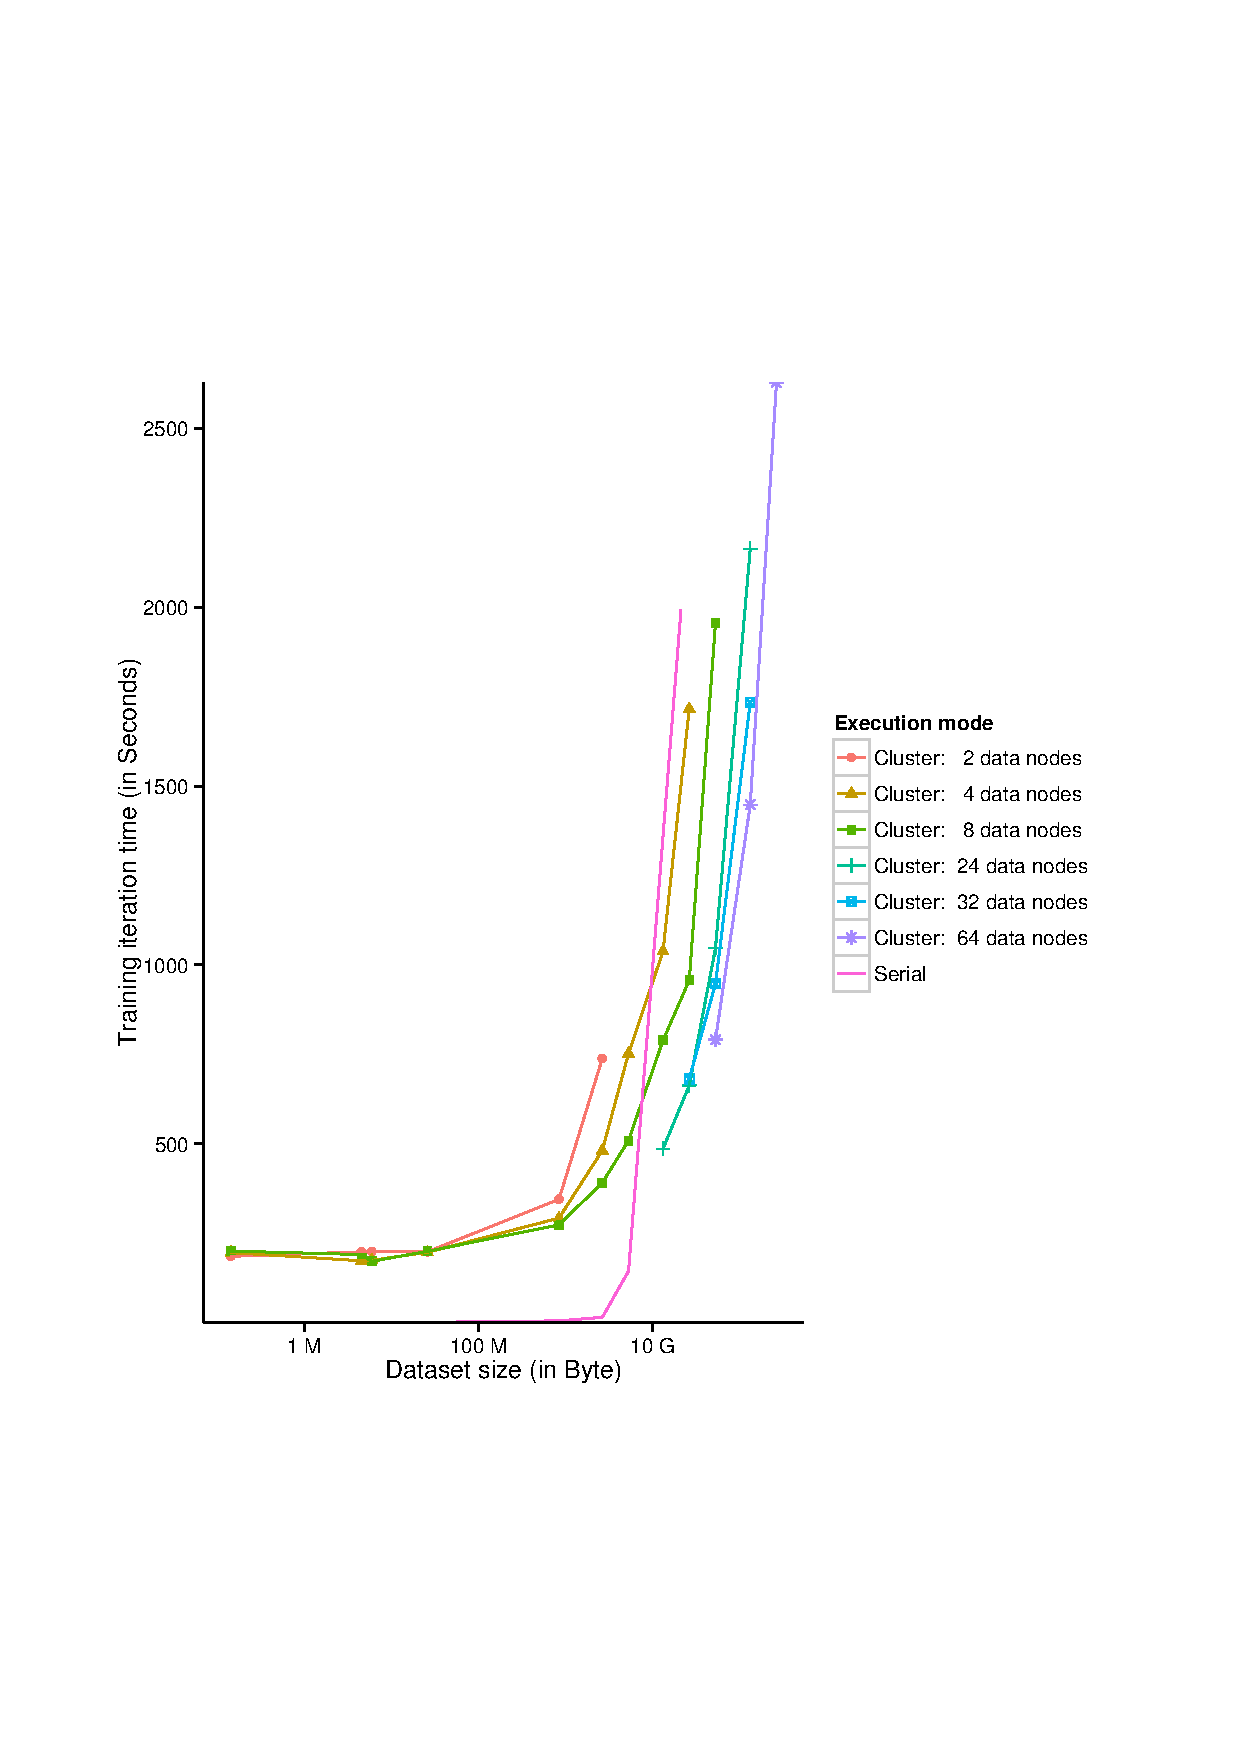
\includegraphics[trim=0cm 5cm 0cm 5cm, scale=0.8]{gfx/time_single_logx.pdf}
\caption{Processing time of a single ListNet training iteration on a logarithmic axis}
\label{fig:listnet_train_time_log}
\end{figure}

Figure \ref{fig:speedup_train_time} shows that speed-up is sub-linear such that the training time converges to a constant unit of time somewhere within the range of 150-200 seconds. This time is likely to be caused by Hadoop job scheduling overhead, this presumption is strengthened by long waiting periods between the separate MapReduce jobs that form a training iteration.\\

Amdahl's law states that the speed-up of a program using parallel computing is limited by the time needed for the sequential fraction of the program. A consequence of Amdahl's Law is that all parallel programs the have a non-parallelisable part have sub-linear speed-up. Behaviour in accordance with Amdahl's law can be seen in Figure \ref{fig:speedup_train_time}, where the speed-up is sub-linear as a result of the existence a non-parallelisable fraction of the program.\\

Note however that Hadoop job scheduling overhead is independent of dataset size. Therefore, the non-parallelisable fraction of the program will be smaller when the to be processed dataset is larger, allowing larger speed-up values for larger datasets. From this observation we can derive that for \emph{"large enough"} datasets, the speed-up obtained by parallelising ListNet using Hadoop MapReduce is large enough for the parallelisation to be beneficial in terms of processing time compared to the RankLib single-machine version of ListNet, even when the size of the to be processed dataset would not have been memory-bounded in RankLib ListNet.\\

Figure \ref{fig:listnet_throughput} shows the throughput in bytes per second. Our observation that RankLib ListNet performs very slow for data sets that do not fit in physical memory and virtual memory is needed is very notable in this graph. Furthermore, this graph shows how both increase in number in data nodes in a cluster and increase in input data size result in an increase in throughput. The sub-linear growth of throughput as a factor of input data size can again be explained as a result of the non-parallelisable Hadoop job scheduling part of the operation.\\

\begin{figure}[!h]
\centering
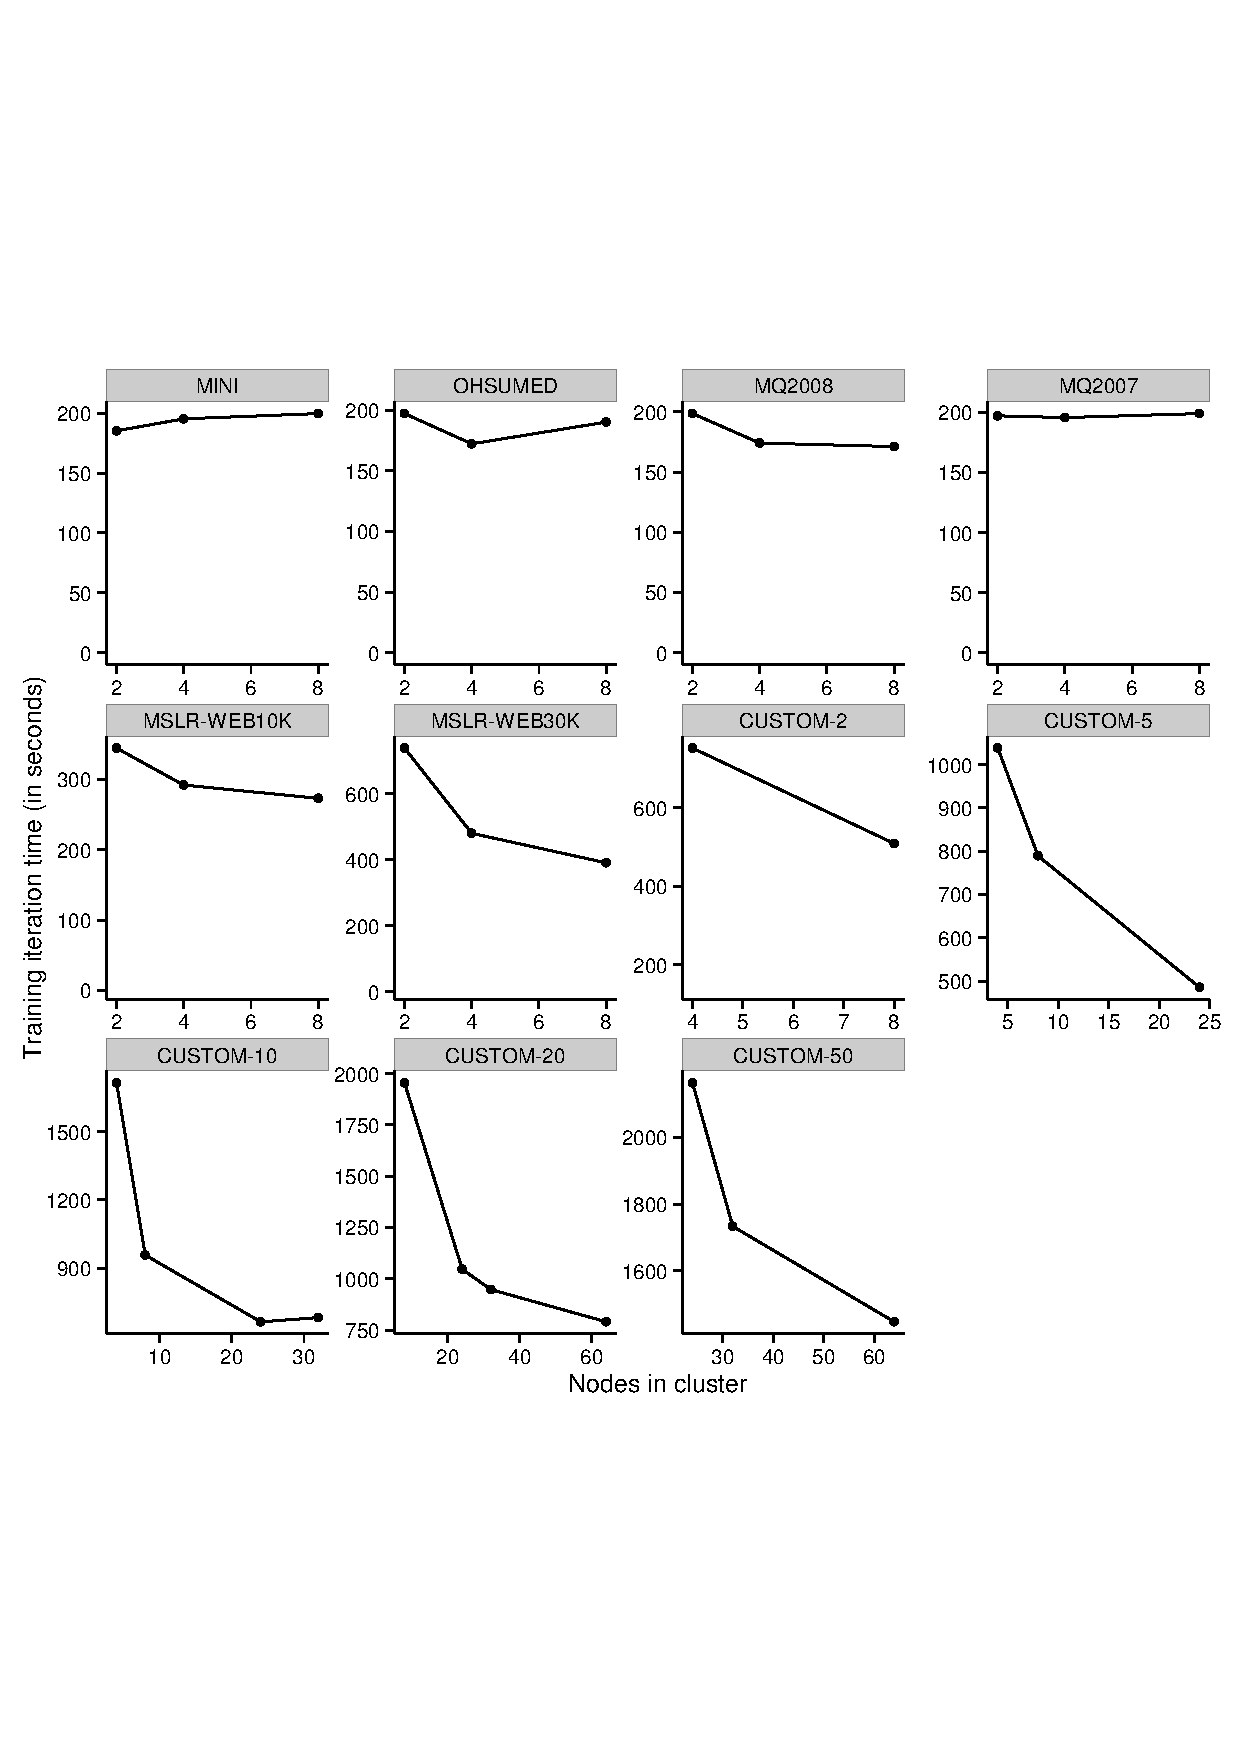
\includegraphics[trim=0cm 5cm 0cm 5cm, scale=0.7]{gfx/speedup_faceted.pdf}
\caption{Processing time as a function of data nodes in a cluster}
\label{fig:speedup_train_time}
\end{figure}

\begin{figure}[!h]
\centering
\includegraphics[trim=0cm 5cm 0cm 5cm, scale=0.8]{gfx/throughput_single_logx.pdf}
\caption{Throughput of a ListNet training iteration}
\label{fig:listnet_throughput}
\end{figure}